\chapter{Graphics Processing Units} \label{chapter:graphics_processing_units}

In this work, we aim to accelerate the execution of our solver using a relatively new architecture,
GPUs. GPUs are massively parallel computer chips that have recently started to be used in the
scientific computing domain. GPUs have initially been used to compute graphical computations, such
as the output to a computer screen, video processing, and synthetic image generation. These
computations are \textit{embarrassingly parallel}, meaning that they are comprised of many identical
computations independent of each other. GPUs are therefore optimised for parallel efficiency.
Combined with the fact that these problems deal with huge amounts of data, GPUs are also optimised
for maximum bandwidth. They are significantly different from \textit{Central Processing Units
(CPUs)}, the traditional architecture on which code is run. CPUs are optimised to solve serial
problems as fast as possible, meaning the prioritise serial speed over parallel efficiency, and
latency over bandwidth. 

Solving fluid flows over a mesh is a parallel problem, as at most steps it is possible to compute
the solution on the different elements making up the mesh in parallel. On the other hand, elements
must exchange information at their interfaces at each time step, meaning careful synchronisation
will be needed. Finally, the adaptivity process detailed in
Chapter~\ref{chapter:adaptive_mesh_refinement} and the load balancing process from
Chapter~\ref{chapter:load_balancing} are not inherently parallel processes. A lot of effort will
have put into breaking up these algorithms into parallel tasks to be run on GPUs. Overall, if it is
possible to efficiently parallelise these sequential parts of the problem, the gains from running
the main solving loop on the highly parallel GPUs should incur a significant speedup to the program.

\section{Architecture} \label{section:graphics_processing_units:architecture}
\subsection{Hardware model} \label{section:graphics_processing_units:architecture:hardware_model}

\begin{figure}[H]
	\centering
	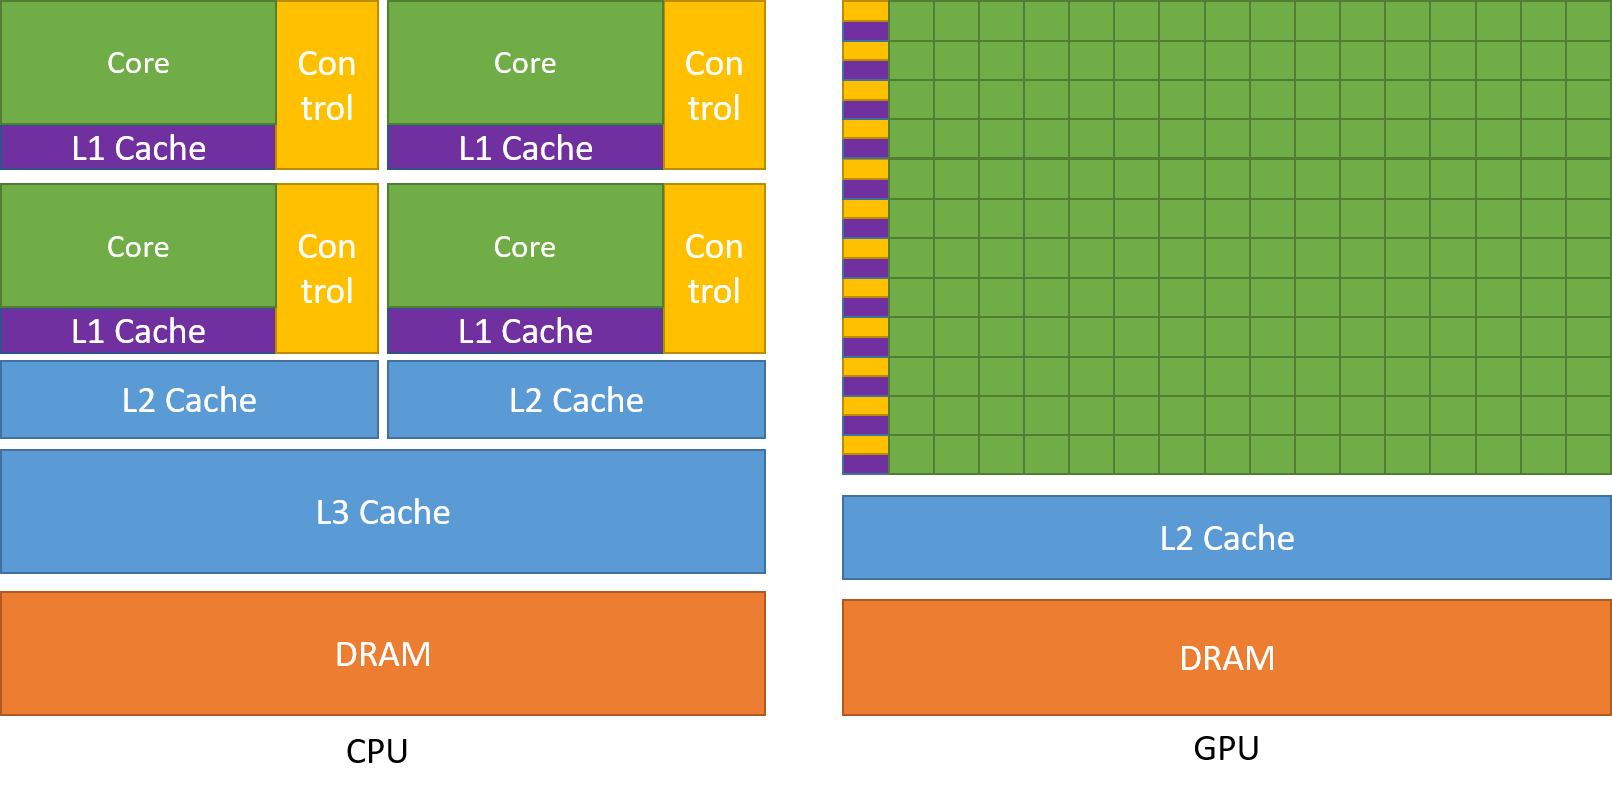
\includegraphics[width=0.8\textwidth]{Chapter_graphics_processing_units/media/gpu-devotes-more-transistors-to-data-processing}
	\caption{CPU and GPU architecture~\cite{Nvidia2021}: GPUs dedicate more space to data processing}
	\label{fig:cpu_gpu}
\end{figure}

Graphics processing units and central processing units are fundamentally made up of the same core
components. First, data processing hardware is shown in green. These are the parts of the chips that
do calculations on data. Then, in yellow is control flow. Control flow hardware schedules
instructions to be executed on processing hardware. In orange is the main memory of either
architecture. Main memory stores data to be used for computations. It is very big, and takes
relatively long to access. Finally, in blue and purple is different levels of cache. Cache is much
smaller and much faster than main memory, and as such stores parts of the memory that the processing
hardware is actively using in order to speed up access.

The two architectures differ as to the balance between the size and capacities of those components.
Chip area is limited by the processes used to manufacture them, so the different components must
share this limited spaces, and sacrifices must be made. GPUs dedicate much more space to data
processing, increasing throughput. Their compute units are also smaller, to work on more data in
parallel. CPUs, on the other hand, have fewer bigger compute units with a higher clock speed in
order to reduce latency. Their compute units are called cores. The GPU compute units are called CUDA
cores, and are arranged in rows as \textit{Streaming Multiprocessors (SMs)}.

In order to reduce latency, CPUs have a lot of die space dedicated to cache. More cache helps keep
data close in access time. More data is loaded from main memory at a time, assuming that data that
is near needed data will also be needed later. The deeper hierarchy of cache of CPUs helps keep the
cores working on the current as fast as possible, never starving for memory. GPUs have less total
cache and fewer levels of cache to make room for more CUDA cores. As a throughput oriented device,
it is less important how fast individual tasks complete, as long as more tasks overall are
completed. The reduced cache is acceptable because if a CUDA core is waiting on data from the main
memory that was not found in cache, it will simply pause execution of that thread and execute
another thread. On GPUs, the smallest and fastest cache, L1 cache, is shared within a SM. It is thus
fast to access shared data, as long as conflicts are avoided.

Finally, CPUs also reduce latency by using much more potent control flow units. Firstly, they have
one control flow unit per core, where GPUs have one control flow unit per row of cores. This limits
how many instruction can be dispatched to the cores making up a SM. The cores will therefore execute
the same execution at the same time in groups of 32, called warps. This makes branching much more
expensive if it happens within a warp. If a part of a program has two branches, A and B, the cores
executing branch A will execute, followed by the cores executing branch B. These have to be executed
sequentially because the control flow unit can only dispatch one instruction per warp. This
multiplies the computation time by the number of taken branches. CPU cores only execute a single
branch, or can even execute both branches at once while waiting for the result of the conditional,
keeping only the correct result once the conditional has been evaluated. The more powerful control
flow units of CPUs may also perform branch prediction, consisting of the CPU guessing the most
likely branch based on the result of previous computations and starting to execute this branch while
waiting for the conditional. All this is performed as an effort to reduce latency as much as
possible. Programs running on GPUs must compensate by avoiding divergence as much as possible within
warps.

\subsection{Programming model} \label{section:graphics_processing_units:architecture:programming_model}

This work uses the CUDA programming model. It is a programming language, framework and runtime to
enable programming on GPUs with an extension of the C++ language. Programs using the language
execute on the CPU like a normal program, but can schedule parts of the program, called kernels, to
be executed on the GPU. Kernels are run in parallel on the GPU, asynchronously from the CPU. The CPU
is therefore free to do computations of its own while the GPU is executing, including adding more
kernels or transfers to the GPU execution queue. Multiple such queues, called streams, can exist.
The purpose of using multiple streams is to execute independent computations on the GPU
concurrently, and maximise GPU usage in case a stream is waiting. GPUs can concurrently execute
kernels, transfer data from the CPU to the GPU, and transfer data from the GPU to the CPU. These
transfers are necessary because CPU and GPU main random access memory are separate. This means that
data needed for computations on the GPU that cannot be generated on it must be explicitly
transferred from the CPU, and results living on the GPU must be transferred bact to the CPU in order
to be displayed or written to disk. As GPUs are also generally running the displays of non-server
computers, results that are only meant to be viewed can be directly displayed and skip such
transfers. This is not the case for this work.

\begin{figure}[H]
	\centering
	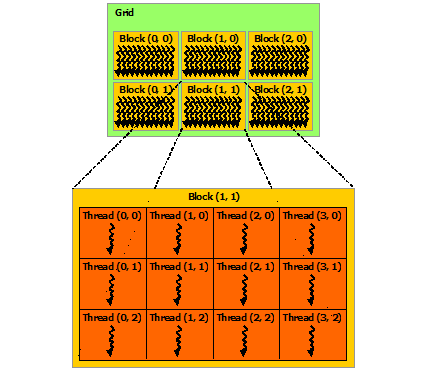
\includegraphics[width=0.6\textwidth]{Chapter_graphics_processing_units/media/grid-of-thread-blocks}
	\caption{GPU programming model~\cite{Nvidia2021}: Execution is split into multiple parallelism levels}
	\label{fig:gpu_programming_model}
\end{figure}

The programing model ties in with the hardware model from
Subsection~\ref{section:graphics_processing_units:architecture:hardware_model} by decomposing the
execution of kernels to multiple parallel levels. A kernel will be executed in parallel, with each
core executing the same function. The whole problem to be solved it the grid. The kernel will
execute until the whole grid has been computed. The grid is broken up into blocks of threads. The
different blocks will be dispatched to the streaming multiprocessors of the GPU, and each thread of
that block will be executed on a CUDA core of the SM. A SM can execute multiple blocks at the same
time if there are more cores within the SM than threads within a block. Blocks need to be completely
independent of each other, as they cannot be synchronised and may execute in any order. They also
cannot share local memory, as each SM has its own L1 cache. Threads within the same block can depend
on one another, as they are executed concurrently on the same SM. Threads from a block execute the
same instruction at the same time in groups of 32, or warps. If there are more threads within a
block than cores within a SM, warps will be run sequentially until all threads are done with the
instruction. Threads within a block can share local memory, and synchronise with each other. This is
useful for algorithms with steps like reductions, where threads will wait until all threads have
computed one level of the reduction, to use the result of that level for the next one.

Typical execution of a program that adds an array A to an array B and stores the result in an array
C will go as following. The CPU side of the program will create two arrays of data in its memory,
and initialise them as needed. It will then create two arrays of the same size on the GPU using the
CUDA runtime, and transfer the data from the CPU arrays A and B to the GPU arrays. It will then
create a result array C on the GPU, and one on the CPU. It will then launch a kernel on the GPU, 
with pointers to the GPU A and B arrays, and the GPU C array. The number of elements in the vectors
will dictate the size of the execution grid. The number of elements will be split in blocks of
threads of fixed size, for example blocks of 128 threads. The number and size of blocks is given to
the GPU when calling the kernel. The CPU then must wait until the computation is done using a
synchronisation with the CUDA runtime, transfer the data from the GPU C array to the CPU C array,
and display the results. 

This model fits well with many CFD methods, including the DG-SEM used in this work. We work on a
mesh made up of elements and faces connecting them. Elements are independent during most of the
computation and can be executed in parallel. The only step from the main solver loop needing extra
care is the computation of the fluxes between the elements. The flux computation uses the data from
the elements on either side of a face, computes a flux and stores that flux back in both elements so
they can compute their derivative. Since there can be multiple faces on each side of an element as
detailed in Section~\ref{section:adaptive_mesh_refinement:mortar_element_method}, and each element
has multiple sides, multiple threads will attempt to read and write to the same locations at the
same time. This is a race condition, where the result of the computation will be dependent on the
order the threads will try to access the memory location. The results may also be wrong. If
two threads read a value, add their contribution, and store the value, only whichever thread wrote
its result last will have its contributed accounted for in the final result. Different approaches
are possible to solve this issue. For example, Giuliani and Krivodonova~\cite{Giuliani2019} use an
edge colouring method where the same kernel is run multiple times on different edges in order to
avoir writing to the elements at the same time. Our program parallelises this part of the
computation on the faces connecting the elements instead, as described in
Section~\ref{section:spectral_element_method:implementation}. As long as there are enough elements
in the mesh to saturate the cores of the GPU with work, this part of the program should e efficient
to run on the GPU.

The adaptivity and load balancing algorithms showed in
Chapters~\ref{chapter:adaptive_mesh_refinement} and~\ref{chapter:load_balancing} are not so easily
parallelisable. These algorithms are sequential in nature, with many operations needing the result
of previous ones to complete. In order to parallelise them, a few support structures have to be
added for the different processing threads to be able to find the data they have been assigned, and 
the different memory locations they are allowed to access. Another issue is that a kernel operating 
on certain objects, elements for example, shouldn't modify other objects, such as faces. This is 
done to avoid race conditions when multiple threads try to access the same memory location, faces in
this example. The practical consequence of this is that objects moving to a new index in their 
storage arrays cannot update their neighbour faces to point to their new index. Their neighbours 
must therefore have the required information to compute where the element will move when the face 
moves itself, and update the index itself. By designing the algorithms this way, a kernel running on 
an object type will have each thread writing to only a single object corresponding to its index, 
avoiding race conditions. More information on how the algorithms are designed is available in 
Sections~\ref{section:spectral_element_method:implementation},
\ref{section:adaptive_mesh_refinement:implementation} and 
\ref{section:load_balancing:implementation}.

The results of load balancing and mesh refinement are also not naturally suited for GPUs. These
processors are more suited for static repetitive tasks. Elements splitting, changing their
polynomial order and moving around will reduce the efficiency of the computations if care is not
taken to tune the algorithms to this platform. Different polynomial orders elements in a thread warp
will introduce branching, and the warp will take as much time to execute as the highest polynomial
order elements. Elements moving around and splitting will put more pressure on the limited cache of
GPUs, as threads will loop on different elements after refinement and load balancing. The interval
between each refinement and load balancing will have to be tuned to trade off between having an
optimal mesh and having a static mesh fore more iterations.

\section{Process Parallelism} \label{section:graphics_processing_units:process_parallelism}
% GPU partitions
% Say something about worker processes, to be general with cpu workers.

When trying to solve very large problems, a single node with a single GPU will have insufficient
processing power and memory to solve the problem in a reasonable time, or at all. To work with these
larger problems, the work needs to be split at another level than GPU parallelism.  

The program can use multi-block meshes, with each block being worked on by one process and one GPU.
If there are fewer GPUs available on a system than there are processes, some processes will share a
single GPU by using asynchronous execution streams. The different processes communicate together
using \textit{Message Passing Interface (MPI)} at their boundaries. Since the solution data resides
on the GPU, it must first be copied to the main CPU memory before it is sent through the MPI
runtime. It then needs to be copied to the receiving process' GPU. This exchange necessitates
multiple transfers on different levels and should be optimised as much as possible. An approach to
minimise the number of interfaces between the different mesh blocks is explained in
Chapter~\ref{chapter:load_balancing}. 

It is possible to split the mesh in more blocks than there are GPUs in a system. In this case, there
will be one process per block, and some processes will share GPUs. The GPUs will be split into
virtual partitions, using concurrent execution streams. These streams execute concurrently on a GPU,
leveraging the fact that some operations can happen at the same time, up to one running kernel, one
transfer from the CPU to the GPU, and one transfer from the GPU to the CPU. Additionally, the GPU
can execute one kernel while another kernel is waiting for memory. These partitions do not increase
performance, but are useful to test running more blocks than there are available GPUs, or running
the program with a mesh that is split in more blocks than available GPUs without re-splitting it.

A simple mesh generator program and a mesh partitioner are available as part of this work. The mesh
generator can create square meshes of arbitrary resolution with different boundary conditions. The
mesh partitioner can split arbitrary single block meshes to multi-block meshes.

These workers, each having a mesh block, do not necessarily need to run on GPUs. A CPU version of
the program is provided to compare the efficiency of the program and to aid debugging. That version
uses CPU workers doing the same computations. The program could even be modified to dispatch work to
CPU and GPU workers to use the full computing power of a system. Some work would need to be done to
ascertain the relative capacity of the different workers, as a GPU worker running on a complete GPU
is much faster than a CPU worker running on a single CPU core. CPU workers could also use multiple
threads, with an architecture similar to the GPU one.

\section{Data structure} \label{section:graphics_processing_units:data_structure}

\begin{figure}[H]
	\centering
	\subfloat[First mesh block]
	{\includesvg[height=0.55\textwidth]{Chapter_graphics_processing_units/media/mesh_0_after0_P2} \label{fig:mesh_left}}
	\hfill
	\subfloat[Second mesh block]
	{\includesvg[height=0.55\textwidth]{Chapter_graphics_processing_units/media/mesh_1_after0_P2} \label{fig:mesh_right}}
	\caption{Data structure: A mesh split into two blocks (a) First block (b) Second block}
	\label{fig:mesh_structure}
\end{figure}

The data structure used in this work has been designed to provide good performance on the GPU
architecture, while keeping the ease of use and programming of CPU code. The mesh is unstructured,
made up of elements, faces and nodes.

\subsection{Performance} \label{section:graphics_processing_units:data_structure:performance}

In order to get good performance and fit naturally with the GPU architecture, the different object
are stored as flat one-dimensional arrays on the GPU. The CUDA memory allocation functions are run
on the CPU and return a continuous block of memory on the GPU, and the memory transfers between the
CPU and GPU copy continuous blocks of memory. This matches well with having flat arrays of objects.
Other data structures, like trees, would need multiple memory allocations from the CPU and a kernel
to assemble them in some kind of structure. This would be manageable for a non-adaptive solver as it
would be performed once, but with mesh refinement and load balancing the mesh changes constantly.
With arrays, an array of the new size is allocated and the objects are moved to it. Thanks to the
structure from
Subsection~\ref{section:graphics_processing_units:data_structure:ease_of_programming}, the elements
themselves have a known constant size regardless of polynomial order, and have the bulk of their
size out of the element object, making them fast to move and making the element array smaller. The
flat arrays also reduce indirection and structure the memory accesses. Threads from a kernel
executing on elements directly access the element at their thread index in the element array.

This simplifies greatly transfers between the CPU and GPU, and mesh reallocation when refining or
load balancing. On the other hand, it carries less context on the relation between mesh blocks,
complicating the element exchanges from Chapter~\ref{chapter:load_balancing}. It also means that
elements and faces move around in the arrays as more are added, and their indices must be updated in
other objects linking to them. 

Some data needs to be transferred to the CPU during the computation, such as fluxes between mesh
blocks in different processes, and data to be written to the output files. These transfers use
arrays allocated on the CPU and GPU, and a kernel storing the data into the GPU array. The array can
then be transferred to the CPU, and either written to disk or sent to another CPU and then its GPU.

\subsection{Ease of use} \label{section:graphics_processing_units:data_structure:ease_of_use}

\begin{figure}[H]
	\centering
	\subfloat[Structured mesh]
	{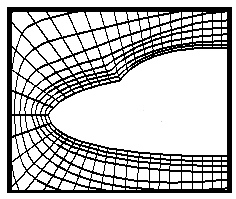
\includegraphics[width=0.45\textwidth]{Chapter_graphics_processing_units/media/structured_mesh} \label{fig:structured_mesh}}
	\hfill
	\subfloat[Unstructured mesh]
	{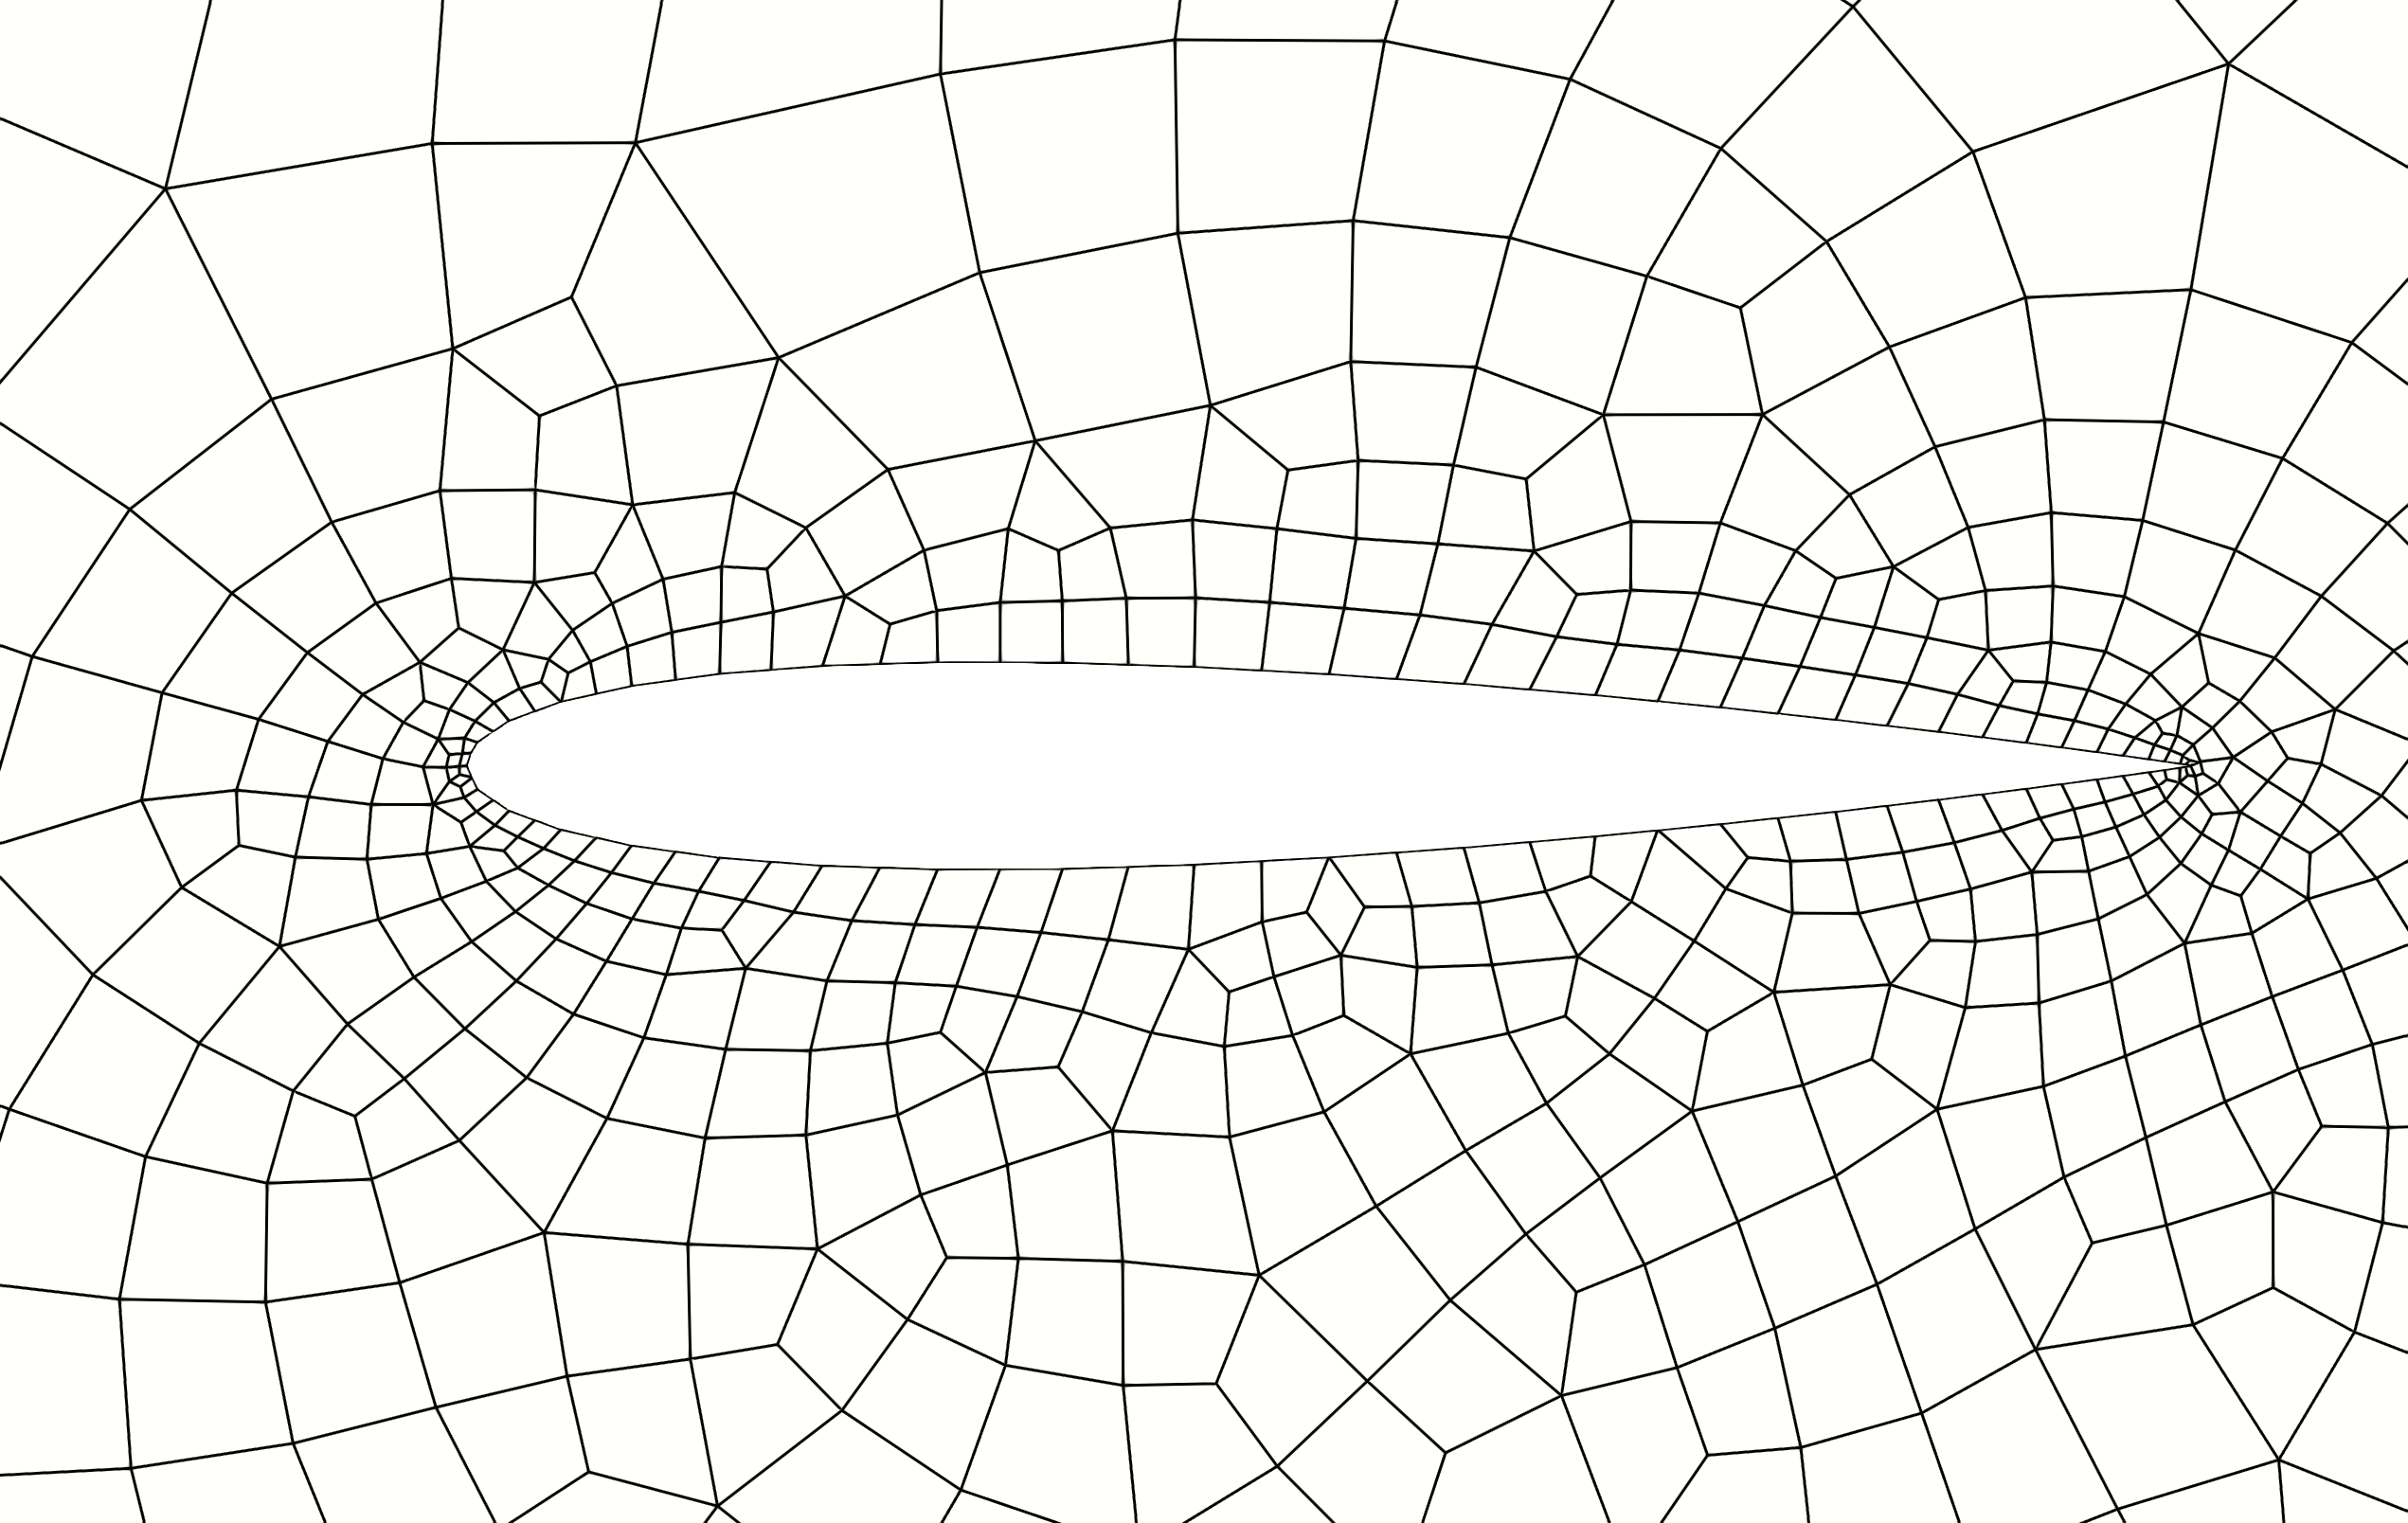
\includegraphics[width=0.45\textwidth]{Chapter_graphics_processing_units/media/unstructured_mesh} \label{fig:unstructured_mesh}}
	\caption{Types of meshes~\cite{Clucas1999}: (a) Structured (b) Unstructured}
	\label{fig:mesh_types}
\end{figure}

In order to increase ease of use, the program is made to work with unstructured meshes. Unstructured
meshes allow for increased flexibility when meshing, and an unstructured mesh solver can easily be
made to also read structured meshes. In unstructured meshes, elements are not necessarily numbered
in any order. Elements hold an explicit list of the indices of their neighbours. In structured
meshes, elements are placed in a regular grid, and have an index describing their location. In 2D,
this is the row and column of the element. The neighbours of an element are found by simply
incrementing or decrementing the index.

\begin{figure}[H]
	\centering
	\subfloat[Structured mesh]
	{\includesvg[width=0.5\textwidth]{Chapter_graphics_processing_units/media/structured_memory} \label{fig:structured_memory}}
	\hfill
	\subfloat[Unstructured mesh]
	{\includesvg[width=0.5\textwidth]{Chapter_graphics_processing_units/media/unstructured_memory} \label{fig:unstructured_memory}}
	\caption{Memory accesses: (a) Structured (b) Unstructured}
	\label{fig:mesh_memory}
\end{figure}

Here a concession has been made for flexibility, as structured meshes would be faster than
unstructured meshes on a GPU. Threads on a GPU benefit from accessing memory in an ordered fashion.
With a structured mesh, thread warps need only one memory access to obtain all their neighbours. The
neighbours are packed in memory, and their index can be computed easily by incrementing the element
indices. For unstructured meshes, neighbour indices have to be fetched from an area in memory, and
the neighbours are not guaranteed to be contiguous in memory. This adds an indirection, and may need
multiple memory accesses.

Since unstructured meshes enable more complex meshes to be represented than strictly regular
quadrilaterals, this tradeoff is accepted, and acts as a worst case scenario for the performance of
GPUs.

The program uses the CGNS mesh format. Both the provided mesh generator and mesh partitioner output
the format, and the mesh partitioner and solver can read the format. The format is widely used,
which should enable this program to read the many already available meshes using the format.

The program outputs data using the VTK format. Once again, this is a widely used format, notably
used by the \textit{ParaView} visualisation application. The results of the program should then be
easy to manipulate and display.

\subsection{Ease of programming} \label{section:graphics_processing_units:data_structure:ease_of_programming}

The program is written partly using the Object-oriented paradigm, especially for the data structure
part. Elements, faces and nodes are objects, each with multiple data members and methods. This
groups many parameters together that would be separate arrays otherwise, making it easier to program
and keep track of the different members of objects. This has the disadvantage of putting more
pressure on the limited cache of GPUs, and potentially increase the number of memory accesses
needed. This is the structure of arrays against array of structures debate. It increases cache
pressure when a loop only accesses a subset of the data members of an object. For example, the
solution update function only used the solution and derivative of an element. When threads loop over
those elements, they have to load entire elements into cache. If the solution and derivative were
stored into separate arrays, much more elements could fit in cache as only their solution and
derivative would be fetched. This would also improve memory accesses, as warps of threads would need
fewer memory accesses since the data is continuous.

On the other hand, using objects simplifies many areas of the code. Elements can be sent and
received from process to process as a whole, adding a data member doesn't necessitate modifying
every part of the code that copies or creates elements. This is especially useful as it enables
using constructors and destructors for objects.

% Figure about dynamic memory

Constructors and destructors are used here because the objects use dynamic memory for their solution
data. As elements and faces can have a different polynomial order, they need to store more or less
data depending on it. This makes it impossible to create an array of objects, unless all objects use
the maximum size they can have, negating the memory advantage of lower-order elements. Instead, in
this work objects use dynamic memory to hold their variable size arrays. They hold pointers to that
memory, making the objects themselves fixed in size. This has the added benefit of making the
objects smaller and easier to move around, as only the pointers and the geometry data have to be
moved while the bigger solution data stays in dynamic memory. 

Unlike the main arrays which are allocated from the CPU on the GPU using the CUDA runtime, GPU
dynamic memory is allocated on the GPU itself. When the elements are created in a kernel, each
thread will allocate memory in parallel in the object constructor. That memory will be deallocated
when the element is deleted. Coupled with move semantics of modern C++, this allows the automatic
management of that memory on the GPU, like we would use smart pointers or arrays in usual C++.
Dynamic memory allocation on the GPU is a relatively new feature, which enables programming patterns
closers to those used for CPU programming.

\section{Implementation} \label{section:graphics_processing_units:implementation}
% Talk about reduce operations, data transfers for boundaries

\subsection{Kernels} \label{section:graphics_processing_units:implementation:kernels}

\subsection{Reductions} \label{section:graphics_processing_units:implementation:reductions}

Reductions are operations that are difficult to make efficient and parallel on GPUs. Harris et
al.~\cite{Harris2007} show a few different ways to optimise these operations. In this work, we need
to compute the minimum time step over the whole mesh at every time step. This operation uses
geometric and solution data from the elements to find each element's minimum time step. This data is
only available on the GPU. 

An implementation must saturate the GPU with work as much as possible, as blindly looping one thread
over the whole mesh will only one of the approximately five thousand cores of the GPU, for one
thousandth of the speed. 